%%==================================================
% CUMTB Thesis for Graduation Project (Undergraduate)  
% Written by ZHAO Xuyang
% version: 0.0.1 (Beta)
%%==================================================


\documentclass[UTF8,AutoFakeBold=1.3,fixskip = true]{ctexart}
	%AutoFakeBold=1.3 设置伪粗,系数1.3,无需添加粗字重的字体
\CTEXoptions[today=old]
\usepackage{appendix}
\usepackage{multirow}
\usepackage{cite}
\usepackage{array}

\usepackage{diagbox}
\usepackage{makecell}

\usepackage{setspace}%调整任意部分的行间距


%引文和目录的超链接====================================
\usepackage{hyperref}
	%删去超链接方框:
	%\hypersetup{colorlinks,linkcolor=black,anchorcolor=black, citecolor=black}


%latex绘图============================================
\usepackage{tikz}
\usetikzlibrary{positioning, shapes.geometric}


%枚举功能=============================================
\usepackage{enumerate}%可以方便的更改item的编号样式
%\usepackage{enumitem}%可以细致的控制item的位置


%插入图片===============================================
\usepackage{graphicx}


%图、表标题设置=========================================
\usepackage{caption}
\usepackage{subcaption}
	\DeclareCaptionFont{songti5bold}{\bfseries\songti\zihao{5}}%自定义字体:宋体、5号、加粗
	\DeclareCaptionFont{songti5}{\songti\zihao{5}}%自定义字体:宋体、5号
	\captionsetup[figure]{font=songti5bold}
	\captionsetup[subfigure]{font=songti5}
%\usepackage{subfigure}%与subcaption冲突,二者取其一


%caption的扩展包,提供中英双语表头、图注====================
%(本科毕设论文不需此功能)
% \usepackage{bicaption}
% \captionsetup[figure][bi-second]{name=Fig.} 
% \captionsetup[table][bi-second]{name=Tab.}


%数学环境================================================
%使用\bm指令对公式中的字符进行加粗
%\mathbf是对公式环境中的文字加粗,会清除公式格式(如斜体等)
\usepackage{bm}
\usepackage{amsmath,amsfonts}


%页面设置,包括纸张、页边距================================
%左右边距均2cm; “装订线位置为左,0.5cm”: left+=0.5cm
\usepackage{geometry}
	%\geometry{margin=1in}
	\geometry{a4paper,left=2.5cm,right=2cm,top=2.5cm,bottom=2.5cm}


%每章图片、表格、公式独立编号==============================
\usepackage{amsmath}
	\numberwithin{figure}{section}
	\numberwithin{table}{section}
	\numberwithin{equation}{section}


%把引用全都变成上标引用=====================================
\makeatletter
\def\@cite#1#2{\textsuperscript{[{#1\if@tempswa , #2\fi}]}}
\makeatother


%插入代码的显示设置========================================
\usepackage{listings}
\usepackage{xcolor}
	\definecolor{dkgreen}{rgb}{0,0.6,0}
	\definecolor{gray}{rgb}{0.5,0.5,0.5}
	\definecolor{mauve}{rgb}{0.58,0,0.82}
	\lstset{
		numbers=left,  
		frame=tb,
		aboveskip=3mm,
		belowskip=3mm,
		showstringspaces=false,
		columns=flexible,
		framerule=1pt,
		rulecolor=\color{gray!35},
		backgroundcolor=\color{gray!5},
		basicstyle={\ttfamily},
		numberstyle=\tiny\color{gray},
		keywordstyle=\color{blue},
		commentstyle=\color{dkgreen},
		stringstyle=\color{mauve},
		breaklines=true,
		breakatwhitespace=true,
		tabsize=3,
	}


%页眉页脚设置=============================================
\usepackage{fancyhdr}
	\pagestyle{fancy}
	\fancyhf{}
	\setlength{\arraycolsep}{1pt}
	\renewcommand{\headrulewidth}{0.1mm}%页眉线宽
	\chead{\songti\zihao{5}~中国矿业大学(北京)2021届本科毕业设计(论文)~}%页眉
	\cfoot{\songti\zihao{5}\thepage}%页脚

	%如此页眉刚好与word的1.5cm,原因尚不明
	%数值越小越靠上
	\setlength{\voffset}{0.4cm}

	% 上页边到页眉的距离 
	%\setlength{\topmargin}{0cm}
	% 标题行高度 
	%\setlength{\headheight}{0.55cm}
	% % 正文到标题的间距
	% \setlength{\headsep}{0.45cm}

	%正文底部到页脚距离,数值越小越靠上
	%此处设置成0.75,页脚到底部距是精确的1.75cm。
	%而此处设置成0.05似乎更符合word结果
	\setlength{\footskip}{0.75cm}

	

%目录页设置================================================
\usepackage{titletoc}

\renewcommand{\contentsname}{\zihao{3} 目\quad\quad 录}
\vspace{1em}

\titlecontents{section}[0em]{\zihao{5}\songti\bf }{\thecontentslabel}{}
{\hspace{.5em}\titlerule*[4pt]{$\cdot$}\contentspage}

\titlecontents{subsection}[2em]{\vspace{0.1\baselineskip}\songti\zihao{5}}
{\thecontentslabel}{}
{\hspace{.5em}\titlerule*[4pt]{$\cdot$}\contentspage}

\titlecontents{subsubsection}[4em]{\vspace{0.1\baselineskip}\songti\zihao{5}}
{\thecontentslabel}{}
{\hspace{.5em}\titlerule*[4pt]{$\cdot$}\contentspage} 



%各级标题设置:===============================================

%选项1:titlesec宏包
% \usepackage{titlesec}
% \titleformat{\section}
% 	[block]
% 	{\zihao{-3}\bfseries\heiti\center}
% 	{\arabic{section} }
% 	{1em}
% 	{}
% \titleformat{\subsection}
% 	[hang]
% 	{}
% 	{\zihao{-3} \thesubsection\enspace}
% 	{0pt}
% 	{\zihao{-3} \bfseries}
% 	[]
% 	{}
% \titleformat{\subsubsection}
% 	[hang]
% 	{}
% 	{\zihao{-4} \thesubsubsection\enspace}
% 	{0pt}
% 	{\zihao{-4} \bfseries}
% 	[]
% 	{}

%选项2:CTeX环境,为了与word排版效果一致,采用了变通设置
	% TeX标题的上下边距独立于标题行距
\CTEXsetup[format={\centering\heiti\zihao{-3}\bfseries}]{section}
\CTEXsetup[beforeskip={1em plus 0.2ex minus 0.2ex}]{section}
\CTEXsetup[afterskip={1em plus 0.2ex minus 0.2ex}]{section}

\CTEXsetup[format={\raggedright\heiti\zihao{4}}]{subsection}
\CTEXsetup[beforeskip={1em plus 0.2ex minus 0.2ex}]{subsection}
\CTEXsetup[afterskip={0.5em plus 0.2ex minus 0.2ex}]{subsection}

\CTEXsetup[format={\raggedright\songti\zihao{-4}\bfseries}]{subsubsection}
\CTEXsetup[beforeskip={0.5em plus 0.2ex minus 0.2ex}]{subsubsection}
\CTEXsetup[afterskip={0em plus 0.2ex minus 0.2ex}]{subsubsection}







%文章开始===========================================================
%===================================================================

\begin{document}

%全文行距、字体、字号控制
\fontsize{12.0pt}{\baselineskip}\selectfont
\setlength{\baselineskip}{25pt}%行间距25磅
\setlength{\parskip}{0pt}%段间距= \parskip + \baselineskip


\begin{spacing}{1.5}
%中文摘要===========================================
\renewcommand{\abstractname}{\zihao{3} 摘\quad\quad 要}
\begin{abstract}
 	\pagestyle{plain}
 	\thispagestyle{empty}%无页眉页脚
	 \zihao{-4}
	\hspace*{\fill} 
	%\vspace{2em}%空两行(无前文也能空)
	\par 摘要内容。
	\\[2em]
	\textbf{关键字}:\quad 关键字1 \quad 关键字2 \quad 关键字3
\end{abstract}

%英文摘要==========================================
\newpage
\ctexset{abstractname = {\songti\zihao{-3} ABSTRACT},}
\begin{abstract}
	\pagestyle{plain}
	\thispagestyle{empty}
	\zihao{-4}
	%\hspace*{\fill} 
	\vspace{1em}
	\par The contents of abstract here.
	\\[2em]
	\textbf{Keywords:}\quad keyword1;\quad keyword2;\quad keyword3

\end{abstract}

\end{spacing}

%目录页=============================================
\newpage
\tableofcontents\thispagestyle{empty}


%正文开始============================================
\newpage
\setcounter{page}{1}%页码计数由此开始

\section{第一章}

	\subsection{第一节}	
		中国矿业大学(China University of Mining and Technology Beijing, CUMTB)\cite{cumtb1909}不同时期的校门,如图\ref{fig:gate}所示。

		%插入双列图片
		\begin{figure}[h!]
			\begin{subfigure}[b]{.5\linewidth}
				\centering
				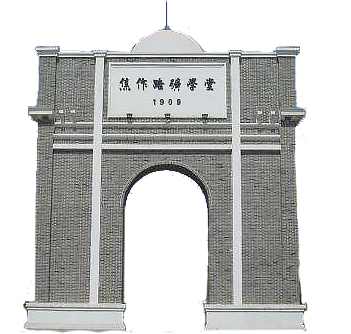
\includegraphics[width=0.5\linewidth]{../pic/lkxt.png}
				\subcaption{路矿学堂}
				\label{fig:1a}
			\end{subfigure}
			\hfill
			\begin{subfigure}[b]{.5\linewidth}
				\centering
				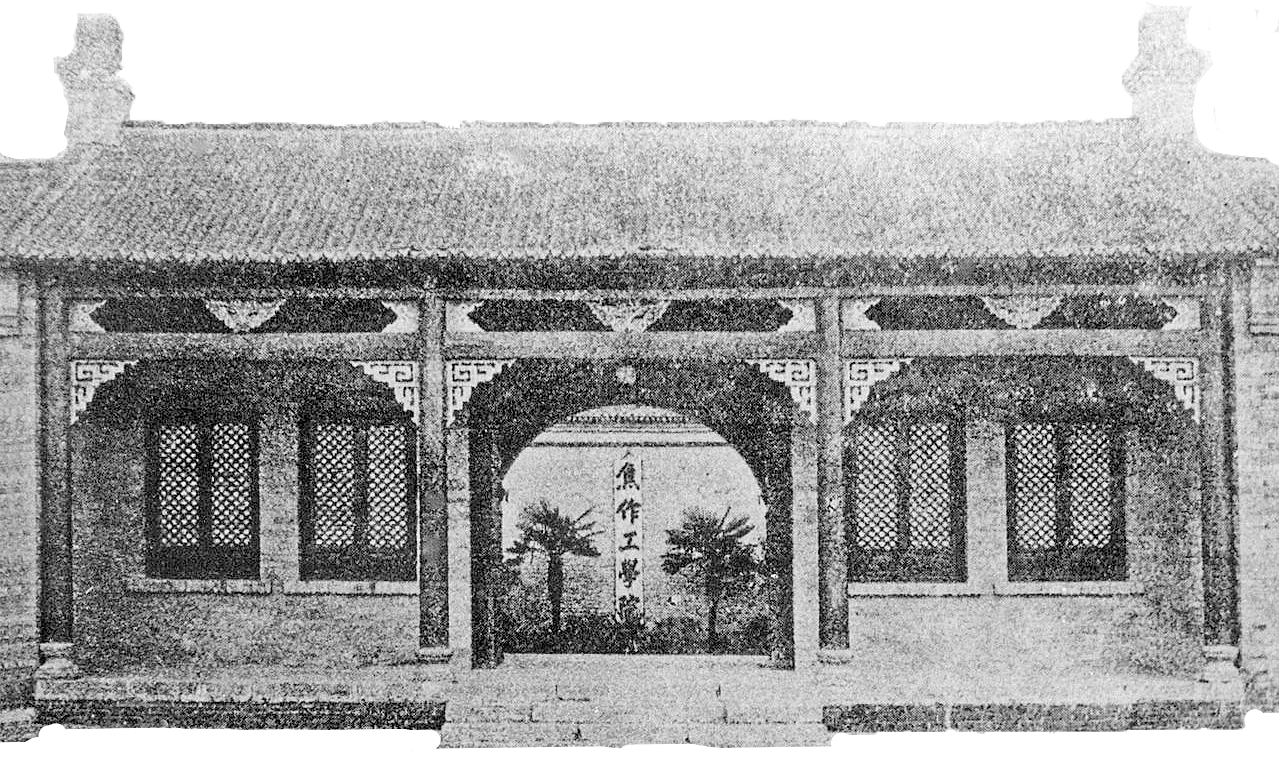
\includegraphics[width=0.7\linewidth]{../pic/jg.png}
				\subcaption{焦作工学院}
				\label{fig:1b}
			\end{subfigure}
			\caption{不同时期的校门}
			\label{fig:gate}
		 \end{figure}
		 

		\subsubsection{第一小节}
		太行之阳河水东,莘莘学子救国重劳工
		\par 源深流自远,物阜民用丰
		\par 山葱葱,水溶溶
		\par 努力,努力
		\par 行健天同功
			\begin{figure}[htbp]
				\centering
				
\includegraphics[width=0.3\linewidth]{../pic/badge.png}
				\caption{校徽}
				\label{fig:badge}
			\end{figure}

\newpage			
\section{第二章}
	\subsection{第一节}	
		中国矿业大学(China University of Mining and Technology Beijing, CUMTB)\cite{cumtb1909}不同时期的校门,如图\ref{fig:gate}所示。

		%插入双列图片
		\begin{figure}[h!]
			\begin{subfigure}[b]{.5\linewidth}
				\centering
				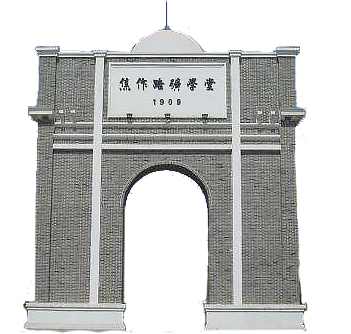
\includegraphics[width=0.5\linewidth]{../pic/lkxt.png}
				\subcaption{路矿学堂}
				\label{fig:1a2}
			\end{subfigure}
			\hfill
			\begin{subfigure}[b]{.5\linewidth}
				\centering
				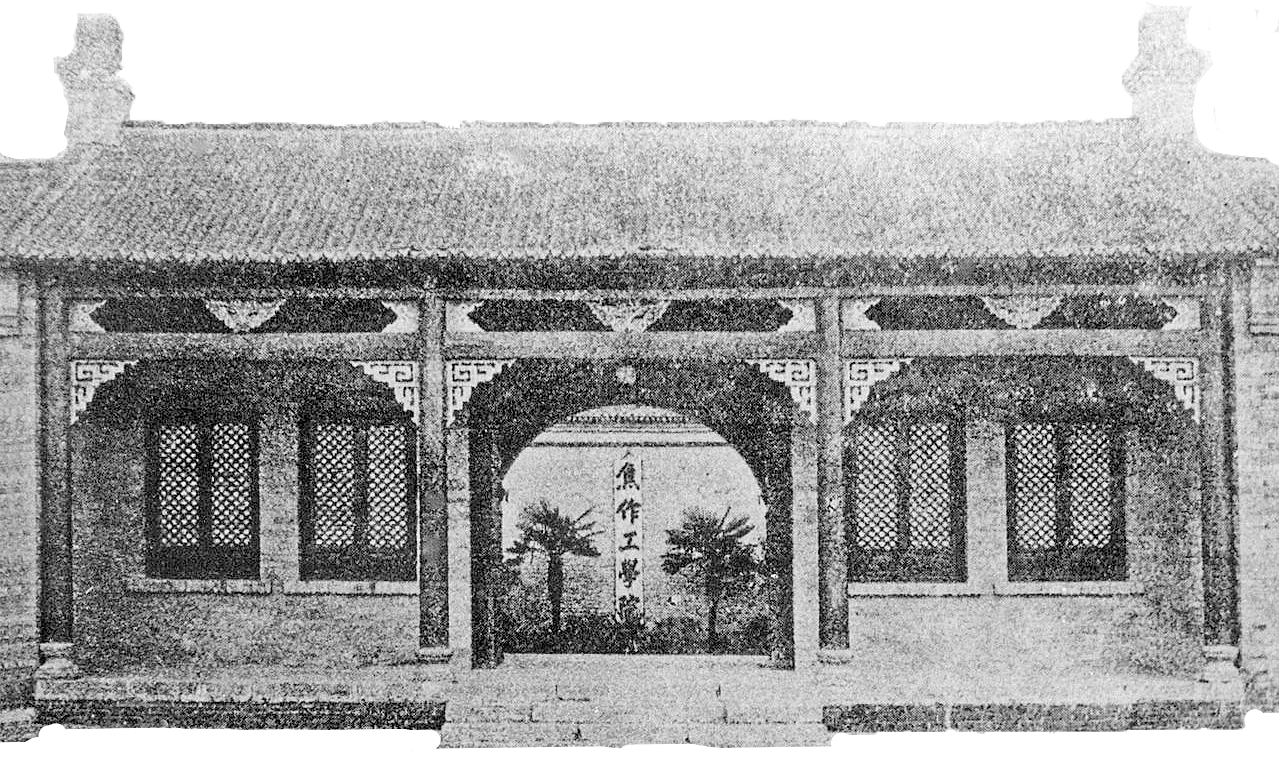
\includegraphics[width=0.7\linewidth]{../pic/jg.png}
				\subcaption{焦作工学院}
				\label{fig:1b2}
			\end{subfigure}
			\caption{不同时期的校门}
			\label{fig:gate2}
		 \end{figure}
		 

		\subsubsection{第一小节}
		\par 努力,努力
		\par 行健天同功
			\begin{figure}[htbp]
				\centering
				
\includegraphics[width=0.3\linewidth]{../pic/badge.png}
				\caption{校徽}
				\label{fig:badge2}
			\end{figure}
		\par 在此插入一个公式\ref{equ:lm1}。
		
		\begin{equation}
			\min _{\Delta \boldsymbol{x}_{k}} \frac{1}{2}\left\|f\left(\boldsymbol{x}_{k}\right)+\boldsymbol{J}\left(\boldsymbol{x}_{k}\right) \Delta \boldsymbol{x}_{k}\right\|^{2}, \quad \text { s.t. }\left\|\boldsymbol{D} \Delta \boldsymbol{x}_{k}\right\|^{2} \leq \mu .
				\label{equ:lm1}
		\end{equation}

\newpage
\section{第三章}
	\subsection{第一节}	
		中国矿业大学(China University of Mining and Technology Beijing, CUMTB)\cite{cumtb1909}不同时期的校门,如图\ref{fig:gate}所示。

		%插入双列图片
		\begin{figure}[h!]
			\begin{subfigure}[b]{.5\linewidth}
				\centering
				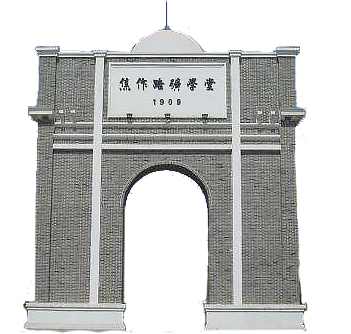
\includegraphics[width=0.5\linewidth]{../pic/lkxt.png}
				\subcaption{路矿学堂}
				\label{fig:1a3}
			\end{subfigure}
			\hfill
			\begin{subfigure}[b]{.5\linewidth}
				\centering
				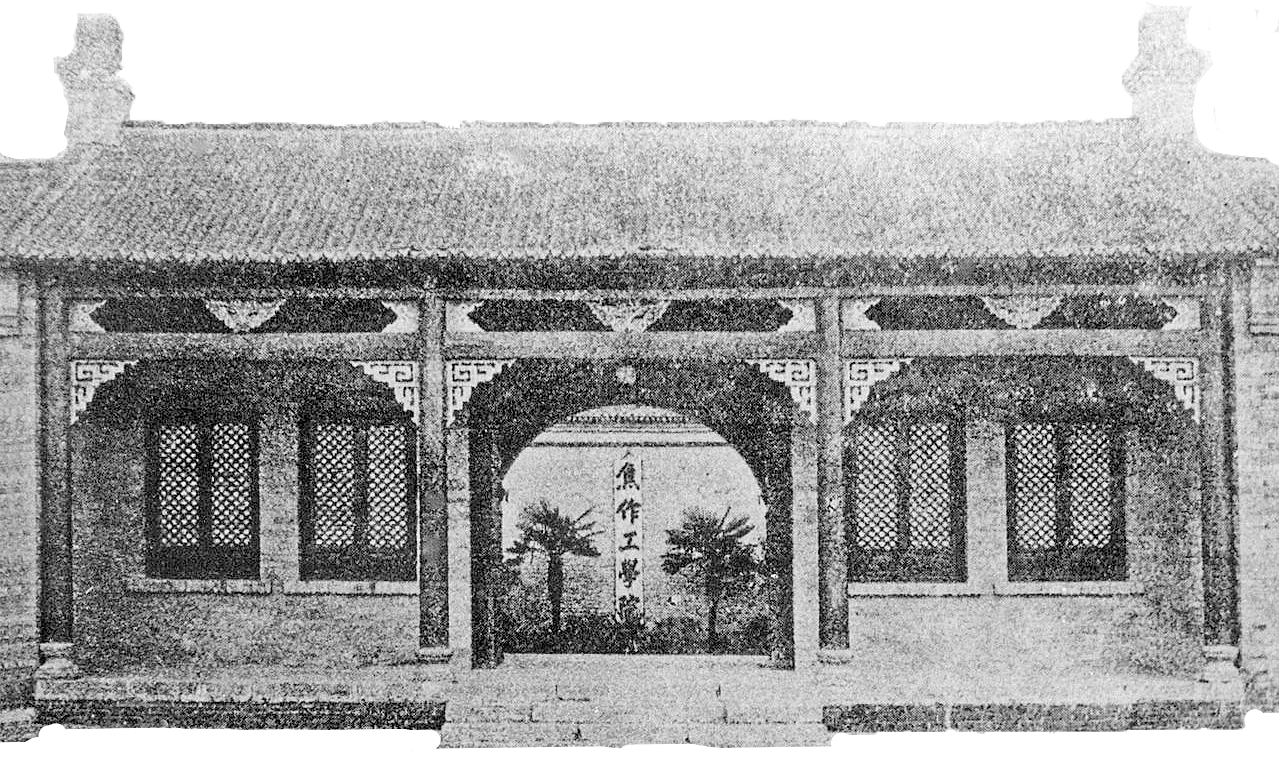
\includegraphics[width=0.7\linewidth]{../pic/jg.png}
				\subcaption{焦作工学院}
				\label{fig:1b3}
			\end{subfigure}
			\caption{不同时期的校门}
			\label{fig:gate3}
			\end{figure}
			

		\subsubsection{第一小节}
		\par 努力,努力
		\par 行健天同功
			\begin{figure}[htbp]
				\centering
				
\includegraphics[width=0.3\linewidth]{../pic/badge.png}
				\caption{校徽}
				\label{fig:badge3}
			\end{figure}
		\par 在此插入一个表格
		
		\begin{table}[h] 
			\caption{实验用平台参数}
			\label{table:param}
			\centering
			\begin{tabular}{p{30pt}p{100pt}p{30pt}p{90pt}p{80pt}}
 			\hline
			\begin{minipage}{3.5cm}\vspace{2mm}设备 \vspace{2mm} \end{minipage} & 系统& RAM & CPU & GPU \\
 			\hline
			\begin{minipage}{3.5cm}\vspace{2mm}笔记本 \vspace{2mm} \end{minipage}  & Ubuntu 18.04   & 64G & i9-10900K 3.7GHz & GeForce RTX 3090 \\
			\begin{minipage}{3.5cm}\vspace{2mm}树莓派 \vspace{2mm} \end{minipage}   & Ubuntu 18.04(ARM) &8G& Cortex-A72 1.5GHz & 无\\
		 	\hline	
			\end{tabular}
		\end{table}




\newpage
\section{总结与展望}
	\subsection{全文工作总结}
		\par 所用\LaTeX 模板于https://github.com/SeanZsya/CUMTB\_Thesis 开放下载。
		\par 
	\subsection{工作展望}
		\begin{enumerate}[\hspace{2em}(1)]
			\item 正文前页面的制作
			\item 编写模板类,接口留出,实现隐去
			\item 证明环境的编辑
			\item 转为 mian.tex-(part.tex)s 的总分模式
			\item 硕士、博士毕业论文制作
		\end{enumerate}



%参考文献=============================================
\newpage
\addcontentsline{toc}{section}{参考文献}%不编号但加入目录
\renewcommand\refname{\bfseries\heiti\zihao{-3} 参考文献} 
\setlength{\baselineskip}{20pt}%行间距20磅
\zihao{5}%文献列表字号:宋体5号

\CTEXsetup[format+={\raggedright}]{section}%标题顶格
\bibliographystyle{GBT7714-2005} %中国GBT7714标准下的引用
\bibliography{../reference/ref} %bib文件
\CTEXsetup[format+={\centering}]{section}

\zihao{-4}%恢复小4号



%致谢==================================================
\newpage
\addcontentsline{toc}{section}{致谢}%不编号但加入目录
\setlength{\baselineskip}{25pt}%行间距25磅
\section*{致谢}
	\par 站在巨人的肩膀上。
	\par Stand on the shoulders of giants.


\end{document}